\documentclass[12pt,titlepage]{article}
\usepackage[margin=1.25in]{geometry}
\usepackage{graphicx,amsmath,blindtext,minted}

%% Variables definition
\newcommand{\vSubject}{Data Structure and Algorithm Practicum}
\newcommand{\vSubtitle}{Stack}
\newcommand{\vName}{Muhammad Baihaqi Aulia Asy'ari}
\newcommand{\vNIM}{2241720145}
\newcommand{\vClass}{1I}
\newcommand{\vDepartment}{Information Technology}
\newcommand{\vStudyProgram}{D4 Informatics Engineering}

%% [START] Tikz related stuff
\usepackage{tikz}
\usetikzlibrary{svg.path,calc,shapes.geometric,shapes.misc}
\tikzstyle{terminator} = [rectangle, draw, text centered, rounded corners = 1em, minimum height=2em]
\tikzstyle{preparation} = [chamfered rectangle, chamfered rectangle sep=0.75em, draw, text centered, minimum height = 2em]
\tikzstyle{process} = [rectangle, draw, text centered, minimum height=2em]
\tikzstyle{decision} = [diamond, aspect=2, draw, text centered, minimum height=2em]
\tikzstyle{data}=[trapezium, draw, text centered, trapezium left angle=60, trapezium right angle=120, minimum height=2em]
\tikzstyle{connector} = [line width=0.25mm,->]
%% [END] Tikz related stuff

%% [START] Fancy header related stuff
\usepackage{fancyhdr}
\pagestyle{fancy}
\setlength{\headheight}{15pt} % compensate fancyhdr style
\fancyhead{}
\fancyfoot{}
\fancyfoot[L]{\thepage}
\fancyfoot[R]{\textit{\vSubject - \vSubtitle}}
\renewcommand{\footrulewidth}{0.4pt}% default is 0pt, overline for footer
%% [END] Fancy header related stuff

%% [START] Custom tabular command related stuff
\usepackage{tabularx}
\newcommand{\details}[2]{
    #1 & #2  \\
}
%% [END] Custom tabular command related stuff

%% [START] Figure related stuff
\newcommand{\image}[3][1]{
    \begin{figure}[h]
        \centering
        \includegraphics[#1]{#2}
        \caption{#3}
        \label{#3}
    \end{figure}
}
%% [END] Figure related stuff

%%
\usepackage{pgf-umlcd}

\renewcommand{\umldrawcolor}{black}
\renewcommand{\umlfillcolor}{white}
%%

%% [BEGIN] Custom enumerator
\usepackage{enumitem}
%% [END] Custom enumerator

%% [START] Arab text
\usepackage{arabtex}
\usepackage{utf8}
\usepackage{unicode}
%% [END] Arab Text

%% [BEGIN] Paragraph indent
\usepackage{indentfirst}
%% [END] Paragraph indent

\begin{document}
\begin{titlepage}
    \centering
    \vfill
    {\bfseries\LARGE
        \vSubject\\
        \vskip0.25cm
        \vSubtitle
    }
    \vfill
    
\includegraphics[width=6cm]{images/polinema-logo.png}
    \vfill
    {
        \textbf{Name}\\
        \vName\\
        \vskip0.5cm
        \textbf{NIM}\\
        \vNIM\\
        \vskip0.5cm
        \textbf{Class}\\
        \vClass\\
        \vskip0.5cm
        \textbf{Department}\\
        \vDepartment\\
        \vskip0.5cm
        \textbf{Study Program}\\
        \vStudyProgram
    }
\end{titlepage}

\newpage

\setcounter{section}{1}
\subsection{Learning Objective}
After finishing this practicum session, students will be able to:

\begin{itemize}
    \item Define the Stack Data Structure
    \item Create and implement Stack Data Structure
    \item Implement Stack data Structure with arrays
\end{itemize}

\subsection{Lab Activities}
In this practicum, we will implement \textbf{Stack} class
\subsubsection{Steps}

\begin{enumerate}
    \item Take a look at this following class diagram for \textbf{Stack} class:
    \mbox{}\\
    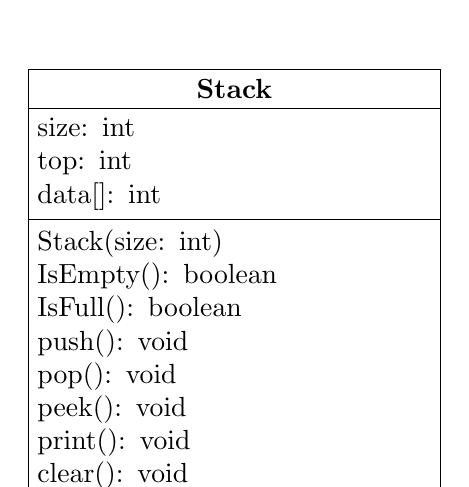
\begin{tikzpicture}
        \begin{class}[text width=5cm]{Stack}{0,0}
            \attribute{size: int}
            \attribute{top: int}
            \attribute{data[]: int}
            \operation{Stack(size: int)}
            \operation{IsEmpty(): boolean}
            \operation{IsFull(): boolean}
            \operation{push(): void}
            \operation{pop(): void}
            \operation{peek(): void}
            \operation{print(): void}
            \operation{clear(): void}
        \end{class}
    \end{tikzpicture}
    \mbox{}\\
    Based on class diagram above, we will create the \textbf{Stack} class in Java program.
    \item Create a new project named \textbf{Jobsheet7}. Create a new package with name \textbf{Practicum1}. Then, create a new class named \textbf{Stack}.
    \item Create new attributes size, top, and data as follows:
    \begin{minted}[autogobble,breaklines]{java}
        int size;
        int top;
        int data[];
    \end{minted}
    \item Add a constructor with parameter as written below:
    \begin{minted}[autogobble,breaklines]{java}
        public Stack(int size) {
            this.size = size;
            data = new int[size];
            top = -1;
        }
    \end{minted}
    \item Create a method \textbf{isEmpty} with Boolean as its return type to check whether the stack is empty or not.
    \begin{minted}[autogobble,breaklines]{java}
        public boolean isEmpty() {
            if (top == 1) {
                return true;
            } else {
                return false;
            }
        }
    \end{minted}
    \item Create a method \textbf{isFull} with Boolean as its return type to check whether the stack is filled completely or not.
    \begin{minted}[autogobble,breaklines]{java}
        public boolean isFull() {
            if (top == size - 1) {
                return true;
            } else {
                return false;
            }
        }
    \end{minted}
    \item Create method \textbf{push} with void as its return type to add new stack element with parameter \textbf{dt}. This dt variable is in form of integer
    \begin{minted}[autogobble,breaklines]{java}
        public void push(int dt) {
            if (!isFull()) {
                top++;
                data[top] = dt;
            } else {
                System.out.println("Stack is full");
            }
        }
    \end{minted}
    \item Create method \textbf{pop} with void as its return type to remove an element from the stack
    \begin{minted}[autogobble,breaklines]{java}
        public void pop() {
            if (!isEmpty()) {
                int x = data[top];
                top--;
                System.out.println("Remove data : " + x);
            } else {
                System.out.println("Stack is empty");
            }
        }
    \end{minted}
    \item Create method \textbf{peek} with void as its return type to check the top element of the stack
    \begin{minted}[autogobble,breaklines]{java}
        public void peek() {
            System.out.println("Top element : " + data[top]);
        }
    \end{minted}
    \item Create method \textbf{print} with void as its return type to display the content of the stack
    \begin{minted}[autogobble,breaklines]{java}
        public void print() {
            System.out.println("Stack content: ");
            for (int i = top; i >= 0; i--) {
                System.out.println(data[i] + " ");
            }
            System.out.println("");
        }
    \end{minted}
    \item Create method \textbf{clear} with void as its data type to remove all elements and make the stack empty
    \begin{minted}[autogobble,breaklines]{java}
        public void clear() {
            if (!isEmpty()) {
                for (int i = top; i >= 0; i--) {
                    top--;
                }
                System.out.println("Stack is now empty");
            } else {
                System.out.println("Failed ! Stack is still empty");
            }
        }
    \end{minted}
    \item Next up, we create a new class named \textbf{StackMain} inside the package \textbf{Practicum1}. Create a main function and make object instantiation with name is \textbf{stk}
    \begin{minted}[autogobble,breaklines]{java}
        public class StackMain {
            public static void main(String[] args) {
                Stack stk = new Stack(5);
            }
        }
    \end{minted}
    \item Fill the stack object by calling method \textbf{push}, the data is being inserted accordingly
    \begin{minted}[autogobble,breaklines]{java}
        stk.push(15);
        stk.push(27);
        stk.push(13);
    \end{minted}
    \item Display the data that we’ve inserted in previous step by calling method \textbf{print}
    \begin{minted}[autogobble,breaklines]{java}
        stk.print();
    \end{minted}
    \item Repeat the insertion process twice, then call pop \textbf{method} to remove an element. We can also check the top data with \textbf{peek} method. Finally, display all the data by calling method \textbf{print}
    \begin{minted}[autogobble,breaklines]{java}
        stk.push(11);
        stk.push(34);
        stk.pop();
        stk.peek();
        stk.print();
    \end{minted}
    \item Compile and run the program, check the result
    \begin{minted}[autogobble,breaklines]{java}
        package Practicum1;

        public class Stack {
            int size;
            int top;
            int data[];

            public Stack(int size) {
                this.size = size;
                data = new int[size];
                top = -1;
            }

            public boolean isEmpty() {
                if (top == 1) {
                    return true;
                } else {
                    return false;
                }
            }

            public boolean isFull() {
                if (top == size - 1) {
                    return true;
                } else {
                    return false;
                }
            }

            public void push(int dt) {
                if (!isFull()) {
                    top++;
                    data[top] = dt;
                } else {
                    System.out.println("Stack is full");
                }
            }

            public void pop() {
                if (!isEmpty()) {
                    int x = data[top];
                    top--;
                    System.out.println("Remove data : " + x);
                } else {
                    System.out.println("Stack is empty");
                }
            }

            public void peek() {
                System.out.println("Top element : " + data[top]);
            }

            public void print() {
                System.out.println("Stack content: ");
                for (int i = top; i >= 0; i--) {
                    System.out.println(data[i] + " ");
                }
                System.out.println("");
            }

            public void clear() {
                if (!isEmpty()) {
                    for (int i = top; i >= 0; i--) {
                        top--;
                    }
                    System.out.println("Stack is now empty");
                } else {
                    System.out.println("Failed ! Stack is still empty");
                }
            }
        }
    \end{minted}
    \begin{minted}[autogobble,breaklines]{java}
        package Practicum1;

        public class StackMain {
            public static void main(String[] args) {
                Stack stk = new Stack(5);

                stk.push(15);
                stk.push(27);
                stk.push(13);

                stk.print();

                stk.push(11);
                stk.push(34);
                stk.pop();
                stk.peek();
                stk.print();
            }
        }
    \end{minted}
\end{enumerate}

\subsubsection{Result}

\begin{minted}[autogobble,breaklines,linenos]{text}
    PS D:\Kuliah>  & 'C:\Program Files\Java\jdk-18.0.2.1\bin\java.exe' '-XX:+ShowCodeDetailsInExceptionMessages' '-cp' 'C:\Users\ASUS\AppData\Roaming\Code\User\workspaceStorage\ ce3fcb236261368a6cbd019dc8ddda8b\redhat.java\ jdt_ws\Kuliah_28156aa7\bin' 'Practicum1.StackMain'
    Stack content: 
    13 
    27
    15

    Remove data : 34
    Top element : 11
    Stack content: 
    11
    13
    27
    15
\end{minted}

\subsubsection{Questions}

\begin{enumerate}
    \item In class \textbf{StackMain}, what is the usage of number 5 in this following code?
    \begin{minted}[autogobble,breaklines]{java}
        Stack stk = new Stack(5);
    \end{minted}
    \texttt{Answer: }
    \mbox{}\\
    the number 5 is used to set the size of the stack
    \item Add 2 more data in the stack with 18 and 40. Display the result!
    \mbox{}\\
    \texttt{Answer: }
    \begin{minted}[autogobble,breaklines]{java}
        package Practicum1;

        public class StackMain {
            public static void main(String[] args) {
                Stack stk = new Stack(5);

                stk.push(15);
                stk.push(27);
                stk.push(13);

                stk.print();

                stk.push(11);
                stk.push(34);
                stk.pop();
                stk.peek();
                stk.print();

                stk.push(18);
                stk.push(40);
            }
        }
    \end{minted}
    \begin{minted}[autogobble,breaklines,linenos]{text}
        PS D:\Kuliah>  & 'C:\Program Files\Java\jdk-18.0.2.1\bin\java.exe' '-XX:+ShowCodeDetailsInExceptionMessages' '-cp' 'C:\Users\G4CE-PC\AppData\Roaming\Code\User\workspaceStorage\ 80d97a47d24665dc0bce7ab1e048ecbd\redhat.java\jdt_ws\ Kuliah_28156aa7\bin' 'Practicum1.StackMain'
        Stack content: 
        13 
        27
        15

        Remove data : 34
        Top element : 11
        Stack content:
        11
        13
        27
        15

        Stack is full
    \end{minted}
    \item In previous number, the data inserted in to the stack is only 18 and 40 is not inserted. Why is that?
    \mbox{}\\
    \texttt{Answer: }
    \mbox{}\\
    Because after pushing the number 18, the stack is already full.
\end{enumerate}

\subsection{2\textsuperscript{nd} Lab Activities}
In this practicum, we will create a program to illustrate a bunch of books that are stored in Stack. Since the book has some information on it, the stack implementation is done using array of object to represent each element.

\subsubsection{Steps}
\begin{enumerate}
    \item This class diagram is used for creating a program code written in Java programming language
    \mbox{}\\
    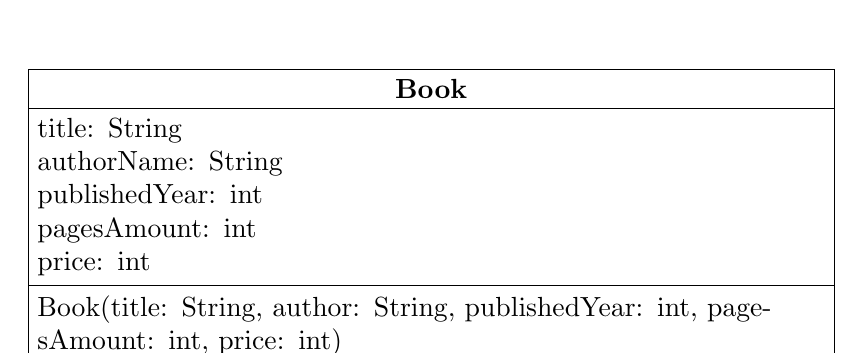
\begin{tikzpicture}
        \begin{class}[text width=10cm]{Book}{0,0}
            \attribute{title: String}
            \attribute{authorName: String}
            \attribute{publishedYear: int}
            \attribute{pagesAmount: int}
            \attribute{price: int}
            \operation{Book(title: String, author: String, publishedYear: int, pagesAmount: int, price: int)}
        \end{class}
    \end{tikzpicture}
    \item Create a new package named \textbf{Practicum2}, then create a new class named \textbf{Book}.
    \item Add attributes in that class, and add the constructor as well.
    \begin{minted}[autogobble,breaklines]{java}
        String title, authorName;
        int publishedYear, pageAmount, price;

        public Book(String tt, String nm, int yr, int pam, int pr) {
            this.title = tt;
            this.authorName = nm;
            this.publishedYear = yr;
            this.pageAmount = pam;
            this.price = pr;
        }
    \end{minted}
    \item Copy the program code for Stack class in \textbf{Practicum1} to be used again in here. Since the data stored in Stack in \textbf{Practicum1} is integer array, and in \textbf{Practicum2} we use objects, we will need to modify some parts in that class.
    \item Modify the Stack class by changing the data type of \textbf{int data[]} to \textbf{Book data[]}. This time we will need to save the data in stack in objects. In addition, we will need to change the \textbf{attributes, constructor, method push}, and \textbf{method pop}
    \begin{minted}[autogobble,breaklines]{java}
        int size, top;
        Book data[];

        public Stack(int size) {
            this.size = size;
            data = new Book[size];
            top = -1;
        }

        public void push(Book dt) {
            if (!isFull()) {
                top++;
                data[top] = dt;
            } else {
                System.out.println("Stack is full");
            }
        }
    \end{minted}
    \item We will need to change the \textbf{print, pop, and peek method} as well since the data that are going to be printed is not only a string, but an object consists of some information (title, authorName, etc.).
    \begin{minted}[autogobble,breaklines]{java}
        public void pop() {
            if (!isEmpty()) {
                Book x = data[top];
                top--;
                System.out.println("Remove data : " + x.title + " " + x.authorName + " " + x.publishedYear + " " + x.publishedYear + " " + x.pageAmount + " " + x.price);
            } else {
                System.out.println("Stack is empty");
            }
        }

        public void peek() {
            System.out.println("Top element : " + data[top]);
        }

        public void print() {
            System.out.println("Stack content: ");
            for (int i = top; i >= 0; i--) {
                System.out.println(data[i].title + " " + data[i].authorName + " " + data[i].publishedYear + " " + data[i].pageAmount + " " + data[i].price);
            }
            System.out.println("");
        }
    \end{minted}
    \item Next, we have to create a new class called \textbf{StackMain} in \textbf{Practicum2}. Create a main function and instantiate an object with named \textbf{st}
    \item Declare the \textbf{Scanner} object with name \textbf{sc}
    \item Insert these lines of codes to receive \textbf{Book} data input, alongside with its information to be stored in stack
    \begin{minted}[autogobble,breaklines]{java}
        Stack st = new Stack(8);
        Scanner sc = new Scanner(System.in);

        char choose;
        do {
            System.out.print("Title : ");
            String title = sc.nextLine();
            
            System.out.print("Author Name : ");
            String name = sc.nextLine();

            System.out.print("Published year : ");
            int year = sc.nextInt();

            System.out.print("Pages Amount : ");
            int pages = sc.nextInt();

            System.out.print("Price : ");
            int price = sc.nextInt();

            Book bk = new Book(title, name, year, pages, price);
            System.out.print("Do you want to add new data to Stack (y/n)? ");
            choose = sc.next().charAt(0);
            sc.nextLine();
            st.push(bk);

        } while (choose == 'y');
    \end{minted}
    \item Call print, pop, and peek method accordingly as follows:
    \begin{minted}[autogobble,breaklines]{java}
        st.print();
        st.pop();
        st.peek();
        st.print();
    \end{minted}
    \item Compile and run \textbf{StackMain}, and observe the result
    \begin{minted}[autogobble,breaklines]{java}
        package Practicum2;

        public class Book {
            String title, authorName;
            int publishedYear, pageAmount, price;

            public Book(String tt, String nm, int yr, int pam, int pr) {
                this.title = tt;
                this.authorName = nm;
                this.publishedYear = yr;
                this.pageAmount = pam;
                this.price = pr;
            }
        }
    \end{minted}
    \begin{minted}[autogobble,breaklines]{java}
        package Practicum2;

        public class Stack {
            int size, top;
            Book data[];

            public Stack(int size) {
                this.size = size;
                data = new Book[size];
                top = -1;
            }

            public boolean isEmpty() {
                if (top == 1) {
                    return true;
                } else {
                    return false;
                }
            }

            public boolean isFull() {
                if (top == size - 1) {
                    return true;
                } else {
                    return false;
                }
            }

            public void push(Book dt) {
                if (!isFull()) {
                    top++;
                    data[top] = dt;
                } else {
                    System.out.println("Stack is full");
                }
            }

            public void pop() {
                if (!isEmpty()) {
                    Book x = data[top];
                    top--;
                    System.out.println("Remove data : " + x.title + " " + x.authorName + " " + x.publishedYear + " " + x.publishedYear + " " + x.pageAmount + " " + x.price);
                } else {
                    System.out.println("Stack is empty");
                }
            }

            public void peek() {
                System.out.println("Top element : " + data[top]);
            }

            public void print() {
                System.out.println("Stack content: ");
                for (int i = top; i >= 0; i--) {
                    System.out.println(data[i].title + " " + data[i].authorName + " " + data[i].publishedYear + " " + data[i].pageAmount + " " + data[i].price);
                }
                System.out.println("");
            }

            public void clear() {
                if (!isEmpty()) {
                    for (int i = top; i >= 0; i--) {
                        top--;
                    }
                    System.out.println("Stack is now empty");
                } else {
                    System.out.println("Failed ! Stack is still empty");
                }
            }
        }
    \end{minted}
    \begin{minted}[autogobble,breaklines]{java}
        package Practicum2;

        import java.util.Scanner;

        public class StackMain {
            public static void main(String[] args) {
                Stack st = new Stack(8);
                Scanner sc = new Scanner(System.in);

                char choose;
                do {
                    System.out.print("Title : ");
                    String title = sc.nextLine();
                    
                    System.out.print("Author Name : ");
                    String name = sc.nextLine();

                    System.out.print("Published year : ");
                    int year = sc.nextInt();

                    System.out.print("Pages Amount : ");
                    int pages = sc.nextInt();

                    System.out.print("Price : ");
                    int price = sc.nextInt();

                    Book bk = new Book(title, name, year, pages, price);
                    System.out.print("Do you want to add new data to Stack (y/n)? ");
                    choose = sc.next().charAt(0);
                    sc.nextLine();
                    st.push(bk);

                } while (choose == 'y');

                st.print();
                st.pop();
                st.peek();
                st.print();
                
                sc.close();
            }
        }
    \end{minted}
\end{enumerate}

\subsubsection{Result}

\begin{minted}[autogobble,breaklines,linenos]{text}
    PS D:\Kuliah>  d:; cd 'd:\Kuliah'; & 'C:\Program Files\Java\jdk-18.0.2.1\bin\java.exe' '-XX:+ShowCodeDetailsInExceptionMessages' '-cp' 'C:\Users\ASUS\AppData\Roaming\Code\User\workspaceStorage\ce3fcb236261368a6cbd019dc8ddda8b\redhat.java\jdt_ws\Kuliah_28156aa7\bin' 'Practicum2.StackMain' 
    Title : Programming
    Author Name : Burhantoro
    Published year : 2016
    Pages Amount : 126
    Price : 58000
    Do you want to add new data to Stack (y/n)? y
    Title : Statistics
    Author Name : Yasir
    Published year : 2014
    Pages Amount : 98
    Price : 44000
    Do you want to add new data to Stack (y/n)? y
    Title : Economics
    Author Name : Diana
    Published year : 2019
    Pages Amount : 86
    Price : 47500
    Do you want to add new data to Stack (y/n)? n
    Stack content: 
    Economics Diana 2019 86 47500
    Statistics Yasir 2014 98 44000
    Programming Burhantoro 2016 126 58000

    Remove data : Economics Diana 2019 2019 86 47500
    Top element : Practicum2.Book@16b98e56
    Stack content:
    Statistics Yasir 2014 98 44000
    Programming Burhantoro 2016 126 58000
\end{minted}

\subsubsection{Questions}

\begin{enumerate}
    \item In class StackMain, when calling \textbf{push} method, the argument is \textbf{bk}. What information is included in the \textbf{bk} variable?
    \mbox{}\\
    \texttt{Answer: }
    \mbox{}\\
    The \textbf{bk} variable contain the title of the book, the author's name, year the book published, the amount of pages in the book, and the price of the book.
    \item Which of the program that its usage is to define the capacity of the stack ?
    \mbox{}\\
    \texttt{Answer: }
    \mbox{}\\
    The capacity of the stack is defined in the instantiation of the stack in the \textbf{StackMain} class as \textbf{st}, which refer to the \textbf{Stack} class.
    \item What is the function of do-while that is exist in \textbf{StackMain} class?
    \mbox{}\\
    \texttt{Answer: }
    \mbox{}\\
    The do-while is used to enter the necessary data for the Book object to be inserted into the stack. After which the user is given the option to add more data or to stop. In this situation the do-while is used to ask the user to atleast input one object, in which after that they are given the option to add more or stop.
    \item Modify the program in \textbf{StackMain}, so that the user may choose which operation (push, pop, peek, print) to do in stack from program menu!
    \mbox{}\\
    \texttt{Answer: }
    \begin{minted}[autogobble,breaklines]{java}
        package Practicum2;

        import java.util.Scanner;

        public class StackMain {
            static Stack st = new Stack(8);
            static Scanner sc = new Scanner(System.in);
            static void callPush() {
                System.out.print("Title : ");
                String title = sc.nextLine();
                
                System.out.print("Author Name : ");
                String name = sc.nextLine();

                System.out.print("Published year : ");
                int year = sc.nextInt();

                System.out.print("Pages Amount : ");
                int pages = sc.nextInt();

                System.out.print("Price : ");
                int price = sc.nextInt();
                
                Book bk = new Book(title, name, year, pages, price);
                st.push(bk);
            }
            public static void main(String[] args) {
                char choose;
                do {
                    System.out.print("Title : ");
                    String title = sc.nextLine();
                    
                    System.out.print("Author Name : ");
                    String name = sc.nextLine();

                    System.out.print("Published year : ");
                    int year = sc.nextInt();

                    System.out.print("Pages Amount : ");
                    int pages = sc.nextInt();

                    System.out.print("Price : ");
                    int price = sc.nextInt();

                    Book bk = new Book(title, name, year, pages, price);
                    System.out.print("Do you want to add new data to Stack (y/n)? ");
                    choose = sc.next().charAt(0);
                    sc.nextLine();
                    st.push(bk);

                } while (choose == 'y');

                /* 
                st.print();
                st.pop();
                st.peek();
                st.print();
                */

                Boolean done = false;
                while (!done) {
                    System.out.println("Which operation would you like to do?");
                    System.out.println("1. push");
                    System.out.println("2. pop");
                    System.out.println("3. peek");
                    System.out.println("4. print");
                    System.out.print("Menu: ");
                    char menu = sc.nextLine().charAt(0);
                    switch (menu) {
                        case '1':
                            callPush();
                            break;
                        case '2':
                            st.pop();
                            break;
                        case '3':
                            st.peek();
                            break;
                        case '4':
                            st.print();
                            break;
                        default:
                            System.out.println("Please insert number as displayed in the menu!");
                            break;
                        }
                    System.out.println("Would you like to do another operation?");
                    System.out.print("Menu (Y/n): ");
                    char option = sc.nextLine().charAt(0);
                    if (option == 'n' || option == 'N') {
                        done = true;
                    }
                }
                sc.close();
            }
        }
    \end{minted}
\end{enumerate}

\subsection{3\textsuperscript{rd} Lab Activities}

In this practicum, we will create program to convert infix notation into postfix notation

\subsubsection{Steps}

\begin{enumerate}
    \item We will use class diagram to create \textbf{Postfix} class in Java program
    \mbox{}\\
    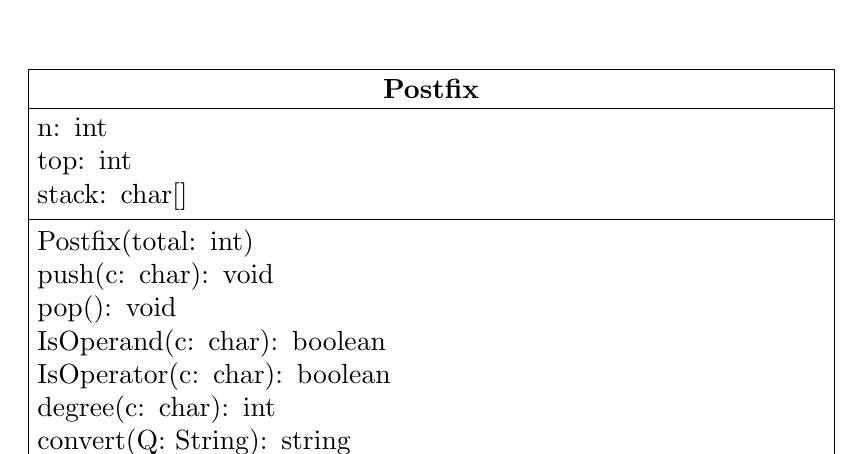
\begin{tikzpicture}
        \begin{class}[text width=10cm]{Postfix}{0,0}
            \attribute{n: int}
            \attribute{top: int}
            \attribute{stack: char[]}
            \operation{Postfix(total: int)}
            \operation{push(c: char): void}
            \operation{pop(): void}
            \operation{IsOperand(c: char): boolean}
            \operation{IsOperator(c: char): boolean}
            \operation{degree(c: char): int}
            \operation{convert(Q: String): string}
        \end{class}
    \end{tikzpicture}
    \item Create a package named \textbf{Practicum3}. Then, we create a new class named \textbf{Postfix}. Add attributes \textbf{n, top, and stack} based on class diagram above.
    \begin{minted}[autogobble,breaklines]{java}
        package Practicum3;

        public class Postfix {
            int n, top;
            char[] stack;
        }
    \end{minted}
    \item Add a constructor with parameter as follows:
    \begin{minted}[autogobble,breaklines]{java}
        public Postfix(int total) {
            n = total;
            top = -1;
            stack = new char[n];
            push('(');
        }
    \end{minted}
    \item Create method \textbf{push} and \textbf{pop} with void as its return type
    \begin{minted}[autogobble,breaklines]{java}
        public void push(char c) {
            top++;
            stack[top] = c;
        }

        public char pop() {
            char item = stack[top];
            top--;
            return item;
        }
    \end{minted}
    \item Create method \textbf{isOperand} as Boolean that will be used to check if the element is operand or not
    \begin{minted}[autogobble,breaklines]{java}
        public boolean isOperand(char c) {
            if ((c >= 'A' && c <= 'Z') || (c >= 'a' && c <= 'z') || (c >= '0' && c <= '9') || c == ' ' || c == '.') {
                return true;
            } else {
                return false;
            }
        }
    \end{minted}
    \item Create method \textbf{isOperator} as booelan that will be used to check if the element is operator or not
    \begin{minted}[autogobble,breaklines]{java}
        public boolean isOperator(char c) {
            if (c == '^' || c == '%' || c == '/' || c == '*' || c == '-' || c == '+') {
                return true;
            } else {
                return false;
            }
        } 
    \end{minted}
    \item Create method \textbf{degree} as integer to define the degree of the operator
    \begin{minted}[autogobble, breaklines]{java}
        public int degree(char c) {
            switch (c) {
                case '^':
                    return 3; 
                case '%':
                    return 2; 
                case '/':
                    return 2; 
                case '*':
                    return 2; 
                case '+':
                    return 1; 
                case '-':
                    return 1; 
                default:
                    return 0;
            }
        }
    \end{minted}
    \item Create method \textbf{convert} to convert infix notation to postfix notation by checking the element one by one in data element.
    \begin{minted}[autogobble,breaklines]{java}
        public String convert(String Q) {
            String p = "";
            char c;
            for (int i = 0; i < n; i++) {
                c = Q.charAt(i);
                if (isOperand(c)) {
                    p = p + c;
                }
                if (c == '(') {
                    push(c);
                }
                if (c == ')') {
                    while (stack[top] != '(') {
                        p = p + pop();
                    }
                    pop();
                }
                if (isOperator(c)) {
                    while (degree(stack[top]) > degree(c)) {
                        p = p + pop();
                    }
                    push(c);
                }
            }
            return p;
        }
    \end{minted}
    \item Next, we will need create a class named \textbf{PostfixMain}. After creating the main function, we create a variable P and Q. P variable will be used to store the final result of converted postfix notation, while Q variable is used to store user input in the form mathematical expression written in infix notation. Instantiate the Scanner object with \textbf{sc} variable, then call build-in \textbf{trim} method to remove spaces within a string.
    \begin{minted}[autogobble,breaklines]{java}
        Scanner sc = new Scanner(System.in);
        String P, Q;
        System.out.println("Insert mathematical expression (infix) : ");
        Q = sc.nextLine();
        Q = Q.trim();
        Q = Q + ")";
    \end{minted} 
    We need to add string \textbf{“)”} to ensure all symbol/ characters that are exist in the stack will be retrieved and moved in postfix.
    \item Create a \textbf{total} variable to calculate how many characters in variable Q
    \begin{minted}[autogobble,breaklines]{java}
        int total = Q.length();
    \end{minted}
    \item Instantiate object \textbf{post} with \textbf{total} as the argument. Then, call \textbf{convert} method to change the infix notation in Q string to postfix notation P
    \begin{minted}[autogobble,breaklines]{java}
        Postfix post = new Postfix(total);
        P = post.convert(Q);
        System.out.println("Postfix : " + P);
    \end{minted}
    \item Compile and run \textbf{StackMain}, and observe the result
    \begin{minted}[autogobble,breaklines]{java}
        package Practicum3;

        public class Postfix {
            int n, top;
            char[] stack;
            
            public Postfix(int total) {
                n = total;
                top = -1;
                stack = new char[n];
                push('(');
            }

            public void push(char c) {
                top++;
                stack[top] = c;
            }

            public char pop() {
                char item = stack[top];
                top--;
                return item;
            }

            public boolean isOperand(char c) {
                if ((c >= 'A' && c <= 'Z') || (c >= 'a' && c <= 'z') || (c >= '0' && c <= '9') || c == ' ' || c == '.') {
                    return true;
                } else {
                    return false;
                }
            }

            public boolean isOperator(char c) {
                if (c == '^' || c == '%' || c == '/' || c == '*' || c == '-' || c == '+') {
                    return true;
                } else {
                    return false;
                }
            }

            public int degree(char c) {
                switch (c) {
                    case '^':
                        return 3; 
                    case '%':
                        return 2; 
                    case '/':
                        return 2; 
                    case '*':
                        return 2; 
                    case '+':
                        return 1; 
                    case '-':
                        return 1; 
                    default:
                        return 0;
                }
            }

            public String convert(String Q) {
                String p = "";
                char c;
                for (int i = 0; i < n; i++) {
                    c = Q.charAt(i);
                    if (isOperand(c)) {
                        p = p + c;
                    }
                    if (c == '(') {
                        push(c);
                    }
                    if (c == ')') {
                        while (stack[top] != '(') {
                            p = p + pop();
                        }
                        pop();
                    }
                    if (isOperator(c)) {
                        while (degree(stack[top]) > degree(c)) {
                            p = p + pop();
                        }
                        push(c);
                    }
                }
                return p;
            }
        }
    \end{minted}

    \begin{minted}[autogobble,breaklines]{java}
        package Practicum3;

        import java.util.Scanner;

        public class PostfixMain {
            public static void main(String[] args) {
                Scanner sc = new Scanner(System.in);
                String P, Q;
                System.out.println("Insert mathematical expression (infix) : ");
                Q = sc.nextLine();
                Q = Q.trim();
                Q = Q + ")";

                int total = Q.length();

                Postfix post = new Postfix(total);
                P = post.convert(Q);
                System.out.println("Postfix : " + P);

                sc.close();
            }
        }
    \end{minted}
\end{enumerate}

\subsubsection{Result}

\begin{minted}[autogobble,breaklines]{text}
    PS D:\Kuliah>  d:; cd 'd:\Kuliah'; & 'C:\Program Files\Java\jdk-18.0.2.1\bin\java.exe' '-XX:+ShowCodeDetailsInExceptionMessages' '-cp' 'C:\Users\G4CE-PC\AppData\Roaming\Code\User\workspaceStorage\ 80d97a47d24665dc0bce7ab1e048ecbd\redhat.java\jdt_ws\ Kuliah_28156aa7\bin' 'Practicum3.PostfixMain' 
    Insert mathematical expression (infix) : 
    a+b*(c+d-e)/f
    Postfix : abcde-+f/*+
\end{minted}

\subsubsection{Questions}

\begin{enumerate}
    \item Please explain the flow of method in Postfix class
    \mbox{}\\
    \texttt{Answer: }
    \mbox{}\\
    The algorithm scan for the problem from the first character. If the algorithm detects an operand, it will put it in the stack. If the algorithm detects an open parentheses, it will put it in the stack. If the algorithm detects a closed parentheses, it will pop trough the stack until it found the open parentheses. If the algorithm detects an operator, then it will check if the stack is empty. If the stack is empty, it will push the operator to the stack. If there is an operator in the stack, it will check if the degree of the operator is bigger than the top of the stack. If it is bigger, the operator will be push. If not, then the stack will be popped until the top of the stack degree is lower than the current operator. If all of the equation has been read. then it will pop everything in the stack. Everytime the stack is popped it will push it to the postfix except for the parentheses.
    \item What is the function of this program code?
    \begin{minted}[autogobble,breaklines]{java}
        c = Q.charAt(i)
    \end{minted}
    \texttt{Answer: }
    \mbox{}\\
    The varibale c is used to store the character the for loop is currently itterating trough the string that has been inputed.
    \item Execute the program again, how’s the result if we insert \textbf{$3 * 5 ^ (8-6) \% 3$} for the expression?
    \mbox{}\\
    \texttt{Answer: }
    \begin{minted}[autogobble,breaklines,linenos]{text}
        PS D:\Kuliah>  & 'C:\Program Files\Java\jdk-18.0.2.1\bin\java.exe' '-XX:+ShowCodeDetailsInExceptionMessages' '-cp' 'C:\Users\G4CE-PC\AppData\Roaming\Code\User\workspaceStorage\ 80d97a47d24665dc0bce7ab1e048ecbd\redhat.java\jdt_ws\ Kuliah_28156aa7\bin' 'Practicum3.PostfixMain'
        Insert mathematical expression (infix) : 
        3*5^(8-6)%3
        Postfix : 3586-^3%*
    \end{minted}
    \item In 2\textsuperscript{nd} number, why the braces are not displayed in conversion result? Please explain
    \mbox{}\\
    \texttt{Answer: }
    \mbox{}\\
    Because in the postfix algorithm, the closed parentheses are only used as limiter to pop trough the stack when the open parentheses is founded. In which both do not get printed.
\end{enumerate}

\subsection{Assignment}

\begin{enumerate}
    \item Create a program with Stack implementation to insert a sentence and display the reversed version of the sentence as a result!
    \begin{minted}[autogobble,breaklines,linenos]{text}
        run:
        Inser Sentence: Politeknik Negeri Malang
        Result : 
        gnalaM iregeN kinketiloP
        BUILD SUCCESSFUL (total time: 1 second)
    \end{minted}
    \begin{minted}[autogobble,breaklines]{java}
        package Assignment1;

        public class Stack {
            int size;
            int top;
            char data[];

            public Stack(int size) {
                this.size = size;
                data = new char[size];
                top = -1;
            }

            public boolean isEmpty() {
                if (top == 1) {
                    return true;
                } else {
                    return false;
                }
            }

            public boolean isFull() {
                if (top == size - 1) {
                    return true;
                } else {
                    return false;
                }
            }

            public void push(char dt) {
                if (!isFull()) {
                    top++;
                    data[top] = dt;
                } else {
                    System.out.println("Stack is full");
                }
            }

            public void pop() {
                if (!isEmpty()) {
                    char x = data[top];
                    top--;
                    System.out.println("Remove data : " + x);
                } else {
                    System.out.println("Stack is empty");
                }
            }

            public void peek() {
                System.out.println("Top element : " + data[top]);
            }

            public void print() {
                System.out.println("Result: ");
                for (int i = top; i >= 0; i--) {
                    System.out.print(data[i]);
                }
            }

            public void clear() {
                if (!isEmpty()) {
                    for (int i = top; i >= 0; i--) {
                        top--;
                    }
                    System.out.println("Stack is now empty");
                } else {
                    System.out.println("Failed ! Stack is still empty");
                }
            }
        }

    \end{minted}
    \begin{minted}[autogobble,breaklines]{java}
        package Assignment1;

        import java.util.Scanner;

        public class StackMain {
            public static void main(String[] args) {
                Scanner sc = new Scanner(System.in);

                System.out.print("Insert Sentence: ");
                String sentence = sc.nextLine(); 

                Stack stk = new Stack(sentence.length());
                for (int i = 0; i < sentence.length(); i++) {
                    stk.push(sentence.charAt(i));
                }
                stk.print();
                
                sc.close();
            }
        }

    \end{minted}
    \begin{minted}[autogobble,breaklines,linenos]{text}
        PS D:\Kuliah>  d:; cd 'd:\Kuliah'; & 'C:\Program Files\Java\jdk-18.0.2.1\bin\java.exe' '-XX:+ShowCodeDetailsInExceptionMessages' '-cp' 'C:\Users\G4CE-PC\AppData\Roaming\Code\User\workspaceStorage\ 80d97a47d24665dc0bce7ab1e048ecbd\redhat.java\jdt_ws\ Kuliah_28156aa7\bin' 'Assignment1.StackMain'    
        Insert Sentence: Politeknik Negeri Malang
        Result: 
        gnalaM iregeN kinketiloP
    \end{minted}
    \item Every Sunday, Dewi shops to a supermarket that is in her residential area. Everytime she finishes, she keeps the receipt of what she has bought in a wardrobe. After 2 months, She had 8 receipts. She plans to trade her 5 receipts in exchange for a voucher. Create a program using stack implementation to store Dewi’s receipt. As well as the retrieving the receipts. The information that are included in a receipt are as follows:
    \begin{itemize}
        \item Transaction ID
        \item Date
        \item Quantity of items
        \item Total price
    \end{itemize}
    \begin{minted}[autogobble,breaklines]{java}
        package Assignment2;

        public class Receipts {
            int transactionID, quantity;
            String date;
            double transactionTotal;

            public Receipts(int transactionID, String date, int quantity, double transactionTotal) {
                this.transactionID = transactionID;
                this.date = date;
                this.quantity = quantity;
                this.transactionTotal = transactionTotal;
            }
        }
    \end{minted}
    \begin{minted}[autogobble,breaklines]{java}
        package Assignment2;

        public class Stack {
            int size, top;
            Receipts data[];

            public Stack(int size) {
                this.size = size;
                data = new Receipts[size];
                top = -1;
            }

            public boolean isEmpty() {
                if (top == 1) {
                    return true;
                } else {
                    return false;
                }
            }

            public boolean isFull() {
                if (top == size - 1) {
                    return true;
                } else {
                    return false;
                }
            }

            public void push(Receipts dt) {
                if (!isFull()) {
                    top++;
                    data[top] = dt;
                } else {
                    System.out.println("Stack is full");
                }
            }

            public void pop() {
                if (!isEmpty()) {
                    Receipts x = data[top];
                    top--;
                    System.out.println("Remove data : " + x.transactionID + " " + x.date + " " + x.quantity + " " + x.transactionTotal);
                } else {
                    System.out.println("Stack is empty");
                }
            }

            public void peek() {
                System.out.println("Top element : " + data[top]);
            }

            public void print(int limit) {
                System.out.printf("last %d data: \n", limit);
                for (int i = top; i >= (size - limit); i--) {
                    System.out.println(data[i].transactionID + " " + data[i].date + " " + data[i].quantity + " " + data[i].transactionTotal);
                }
                System.out.println("");
            }

            public void clear() {
                if (!isEmpty()) {
                    for (int i = top; i >= 0; i--) {
                        top--;
                    }
                    System.out.println("Stack is now empty");
                } else {
                    System.out.println("Failed ! Stack is still empty");
                }
            }
        }
    \end{minted}
    \begin{minted}[autogobble,breaklines]{java}
        package Assignment2;

        public class StackMain {
            public static void main(String[] args) {
                Stack stack = new Stack(8);

                int[] transactionIDs = {1, 2, 3, 4, 5, 6, 7, 8};
                String[] date = {" 7 February 2023", "14 February 2023", "21 February 2023", "28 February 2023", " 7 March 2023", "14 March 2023", "21 March 2023", "28 March 2023"};
                int[] quantity = {5, 7, 8, 6, 7, 7, 5, 6};
                double[] transactionTotal = {85_000, 115_000, 150_000, 100_000, 115_000, 115_000, 85_000, 100_000};

                for (int i = 0; i < stack.size; i++) {
                    System.out.printf("%d %s %d %,.2f\n", transactionIDs[i], date[i], quantity[i], transactionTotal[i]);
                }

                System.out.println();

                for (int i = 0; i < stack.size; i++) {
                    Receipts receipts = new Receipts(transactionIDs[i], date[i], quantity[i], transactionTotal[i]);
                    stack.push(receipts);
                }

                int requestedReceipts = 5;
                stack.print(requestedReceipts);
            }
        }
    \end{minted}
    \begin{minted}[autogobble,breaklines,linenos]{text}
        PS D:\Kuliah>  d:; cd 'd:\Kuliah'; & 'C:\Program Files\Java\jdk-18.0.2.1\bin\java.exe' '-XX:+ShowCodeDetailsInExceptionMessages' '-cp' 'C:\Users\G4CE-PC\AppData\Roaming\Code\User\workspaceStorage\ 80d97a47d24665dc0bce7ab1e048ecbd\redhat.java\jdt_ws\ Kuliah_28156aa7\bin' 'Assignment2.StackMain' 
        1  7 February 2023 5 85,000.00
        2 14 February 2023 7 115,000.00
        3 21 February 2023 8 150,000.00
        4 28 February 2023 6 100,000.00
        5  7 March 2023 7 115,000.00
        6 14 March 2023 7 115,000.00
        7 21 March 2023 5 85,000.00
        8 28 March 2023 6 100,000.00

        last 5 data:
        8 28 March 2023 6 100000.0
        7 21 March 2023 5 85000.0
        6 14 March 2023 7 115000.0
        5  7 March 2023 7 115000.0
        4 28 February 2023 6 100000.0
    \end{minted}
\end{enumerate}

\end{document}